\documentclass[conference]{IEEEtran}
\IEEEoverridecommandlockouts
\usepackage{cite}
\usepackage{amsmath,amssymb,amsfonts}
\usepackage{algorithmic}
\usepackage{graphicx}
\usepackage{textcomp}
\usepackage{xcolor}
\usepackage{hyperref}
\usepackage{booktabs}
\usepackage{multirow}
\usepackage{float}
\usepackage{algorithm}
\usepackage{algpseudocode}
\usepackage{listings}
\usepackage{xcolor}
\usepackage{siunitx}
\usepackage{pgfplots}
\pgfplotsset{compat=1.18}

\definecolor{codegreen}{rgb}{0,0.6,0}
\definecolor{codegray}{rgb}{0.5,0.5,0.5}
\definecolor{codepurple}{rgb}{0.58,0,0.82}
\definecolor{backcolour}{rgb}{0.95,0.95,0.92}

\lstdefinestyle{mystyle}{
    backgroundcolor=\color{backcolour},   
    commentstyle=\color{codegreen},
    keywordstyle=\color{magenta},
    numberstyle=\tiny\color{codegray},
    stringstyle=\color{codepurple},
    basicstyle=\ttfamily\footnotesize,
    breakatwhitespace=false,         
    breaklines=true,                 
    captionpos=b,                    
    keepspaces=true,                 
    numbers=left,                    
    numbersep=5pt,                  
    showspaces=false,                
    showstringspaces=false,
    showtabs=false,                  
    tabsize=2
}

\lstset{style=mystyle}

\def\BibTeX{{\rm B\kern-.05em{\sc i\kern-.025em b}\kern-.08em
    T\kern-.1667em\lower.7ex\hbox{E}\kern-.125emX}}

\begin{document}

\title{Development of an Adaptive Machine Learning-Based Trading Bot with Enhanced Risk Management and Advanced Market Analysis}

\author{\IEEEauthorblockN{Md Safuan Siddik}
\IEEEauthorblockA{Department of Computer Science\\
Goldsmiths University of London\\
Email: msidd002@gold.ac.uk}}

\maketitle

\begin{abstract}
This paper presents the development and implementation of an advanced trading bot that leverages state-of-the-art machine learning techniques for financial market prediction and automated trading. The system incorporates multiple neural network architectures, including Long Short-Term Memory (LSTM) networks and custom neural networks, combined with sophisticated technical analysis indicators for enhanced decision-making. A key innovation is the implementation of adaptive risk management strategies that dynamically adjust based on market conditions, historical performance, and real-time market microstructure analysis. The bot features comprehensive backtesting capabilities with detailed performance metrics, advanced visualization tools, and sophisticated market regime detection algorithms. Through extensive testing and validation across multiple market conditions, the system demonstrates superior performance in automated trading strategies that can adapt to changing market conditions while maintaining strict risk controls.
\end{abstract}

\begin{IEEEkeywords}
Trading Bot, Machine Learning, Risk Management, LSTM, Neural Networks, Financial Markets, Market Microstructure, Adaptive Systems, Portfolio Optimization
\end{IEEEkeywords}

\section{Introduction}
The rapid evolution of financial markets and the increasing complexity of trading strategies have created a growing demand for sophisticated automated trading systems. Traditional trading approaches often struggle to adapt to rapidly changing market conditions and may not effectively incorporate the vast amounts of available market data. This project addresses these challenges by developing an advanced trading bot that combines state-of-the-art machine learning techniques with robust risk management strategies and sophisticated market analysis tools.

\subsection{Motivation}
The development of automated trading systems has become increasingly important due to several factors:
\begin{itemize}
    \item Increasing market complexity and data volume requiring sophisticated analysis
    \item Need for faster and more accurate trading decisions in high-frequency environments
    \item Growing importance of risk management in volatile markets
    \item Potential for improved returns through systematic trading
    \item Demand for consistent performance across market regimes
    \item Evolution of market microstructure and algorithmic trading
    \item Integration of alternative data sources and real-time analytics
    \item Advancement in machine learning and computational capabilities
\end{itemize}

\subsection{Research Objectives}
The primary objectives of this project are:
\begin{itemize}
    \item To develop a machine learning-based trading system capable of predicting market movements with high accuracy
    \item To implement comprehensive risk management strategies that adapt to market conditions
    \item To create a robust backtesting framework for strategy validation
    \item To demonstrate the effectiveness of combining multiple technical indicators with machine learning predictions
    \item To develop advanced market regime detection algorithms
    \item To implement sophisticated portfolio optimization techniques
    \item To investigate the impact of market microstructure on trading decisions
    \item To evaluate the effectiveness of adaptive learning mechanisms
    \item To analyze the relationship between model complexity and performance
    \item To develop efficient real-time processing capabilities
\end{itemize}

\subsection{Contributions}
This work makes several significant contributions to the field:
\begin{itemize}
    \item Novel approach to combining machine learning with technical analysis
    \item Advanced implementation of adaptive risk management
    \item Innovative backtesting methodology
    \item Efficient data processing architecture
    \item Sophisticated market regime detection algorithms
    \item Advanced portfolio optimization techniques
    \item New insights into market microstructure analysis
    \item Enhanced understanding of adaptive learning in trading
    \item Improved methods for real-time data processing
    \item Novel approaches to risk factor decomposition
\end{itemize}

\subsection{Technical Challenges}
The development of the trading bot faced several significant challenges:
\begin{itemize}
    \item Real-time data processing and latency optimization
    \item Model complexity vs. interpretability trade-off
    \item Handling of market microstructure effects
    \item Integration of multiple data sources and timeframes
    \item Development of robust risk management systems
    \item Implementation of efficient backtesting frameworks
    \item Optimization of computational resources
    \item Management of model drift and decay
    \item Handling of market regime transitions
    \item Integration of alternative data sources
\end{itemize}

\subsection{Methodology Overview}
The research methodology encompasses several key components:
\begin{itemize}
    \item Data collection and preprocessing pipeline
    \item Feature engineering and selection process
    \item Model development and validation framework
    \item Risk management system implementation
    \item Backtesting and performance evaluation
    \item Market regime analysis methodology
    \item Portfolio optimization techniques
    \item Real-time processing architecture
    \item Adaptive learning mechanisms
    \item Performance monitoring and analysis
\end{itemize}

\subsection{Expected Impact}
The project's outcomes are expected to have significant implications:
\begin{itemize}
    \item Advancement in algorithmic trading methodologies
    \item Improved risk management practices
    \item Enhanced market efficiency understanding
    \item Better portfolio optimization techniques
    \item More sophisticated market analysis tools
    \item Improved adaptive learning systems
    \item Enhanced real-time processing capabilities
    \item Better understanding of market microstructure
    \item More effective risk factor decomposition
    \item Advanced market regime detection methods
\end{itemize}

\section{Background}
\subsection{Machine Learning in Trading}
The application of machine learning in financial markets has gained significant attention in recent years. Various approaches have been explored, including:

\subsubsection{Neural Networks}
Neural networks have proven particularly effective in financial market prediction due to their ability to:
\begin{itemize}
    \item Learn complex non-linear patterns in market data
    \item Adapt to changing market conditions
    \item Process multiple input features simultaneously
    \item Handle noisy and incomplete data
    \item Capture temporal dependencies in time series
    \item Model complex market dynamics
    \item Integrate multiple data sources
    \item Provide probabilistic predictions
\end{itemize}

\subsubsection{LSTM Networks}
LSTM networks are particularly well-suited for time series prediction due to their:
\begin{itemize}
    \item Ability to capture long-term dependencies
    \item Memory mechanisms for retaining important information
    \item Robustness to noise and missing data
    \item Effectiveness in handling sequential data
    \item Capability to learn complex temporal patterns
    \item Adaptive learning mechanisms
    \item Integration with attention mechanisms
    \item Multi-scale feature extraction
\end{itemize}

\subsubsection{Ensemble Methods}
Ensemble methods combine multiple models to improve prediction accuracy:
\begin{itemize}
    \item Bagging and boosting techniques
    \item Model averaging and stacking
    \item Cross-validation and model selection
    \item Feature importance analysis
    \item Dynamic model weighting
    \item Adaptive ensemble strategies
    \item Multi-timeframe integration
    \item Risk-aware model combination
\end{itemize}

\subsection{Risk Management in Automated Trading}
Effective risk management is crucial for automated trading systems. Key aspects include:

\subsubsection{Position Sizing}
Advanced position sizing strategies consider:
\begin{itemize}
    \item Account equity and risk tolerance
    \item Market volatility and liquidity
    \item Correlation between positions
    \item Portfolio-level risk constraints
    \item Market regime conditions
    \item Historical performance metrics
    \item Real-time risk monitoring
    \item Dynamic adjustment mechanisms
\end{itemize}

\subsubsection{Stop-Loss and Take-Profit}
Sophisticated exit strategies incorporate:
\begin{itemize}
    \item Dynamic threshold adjustment
    \item Multiple exit conditions
    \item Partial profit taking
    \item Trailing stops
    \item Volatility-based adjustments
    \item Market regime adaptation
    \item Time-based exits
    \item Risk-reward optimization
\end{itemize}

\subsubsection{Portfolio Risk Monitoring}
Comprehensive risk monitoring includes:
\begin{itemize}
    \item Maximum drawdown limits
    \item Position concentration limits
    \item Correlation-based risk adjustment
    \item Daily trading limits
    \item Value at Risk (VaR) analysis
    \item Expected Shortfall calculations
    \item Stress testing scenarios
    \item Real-time risk alerts
\end{itemize}

\subsection{Market Microstructure}
Understanding market microstructure is essential for effective trading:

\subsubsection{Order Book Analysis}
Key components include:
\begin{itemize}
    \item Order flow analysis
    \item Liquidity measurement
    \item Price impact modeling
    \item Market depth analysis
    \item Order book imbalance
    \item Spread analysis
    \item Volume profile
    \item Market impact costs
\end{itemize}

\subsubsection{Market Impact}
Important considerations include:
\begin{itemize}
    \item Slippage modeling
    \item Transaction costs
    \item Market liquidity
    \item Order execution strategies
    \item Price impact analysis
    \item Market efficiency
    \item Trading costs
    \item Execution algorithms
\end{itemize}

\subsection{Technical Analysis}
Advanced technical analysis techniques include:

\subsubsection{Price Action}
Key patterns and indicators:
\begin{itemize}
    \item Support and resistance levels
    \item Trend analysis
    \item Chart patterns
    \item Candlestick patterns
    \item Price momentum
    \item Volume analysis
    \item Market structure
    \item Price action strategies
\end{itemize}

\subsubsection{Technical Indicators}
Advanced indicators include:
\begin{itemize}
    \item Moving averages and variations
    \item Oscillators and momentum indicators
    \item Volume-based indicators
    \item Volatility indicators
    \item Trend strength indicators
    \item Market breadth indicators
    \item Custom composite indicators
    \item Adaptive indicators
\end{itemize}

\subsection{Data Analysis}
Sophisticated data analysis techniques include:

\subsubsection{Time Series Analysis}
Key methods include:
\begin{itemize}
    \item Statistical analysis
    \item Trend decomposition
    \item Seasonality analysis
    \item Stationarity testing
    \item Correlation analysis
    \item Cointegration testing
    \item Granger causality
    \item Spectral analysis
\end{itemize}

\subsubsection{Feature Engineering}
Advanced techniques include:
\begin{itemize}
    \item Technical indicator creation
    \item Statistical feature extraction
    \item Domain-specific features
    \item Feature selection methods
    \item Feature interaction analysis
    \item Dimensionality reduction
    \item Feature scaling and normalization
    \item Feature importance analysis
\end{itemize}

\section{Methods}
\subsection{System Architecture}
The trading bot is implemented as a modular system with the following key components:

\subsubsection{Market Data Management}
The Market Data Manager handles:
\begin{itemize}
    \item Real-time data ingestion and processing
    \item Historical data management
    \item Data validation and cleaning
    \item Feature engineering and normalization
    \item Time series alignment and resampling
    \item Robust error checking and latency optimization
\end{itemize}

\subsubsection{Machine Learning Models}
The system implements multiple model architectures:

\paragraph{LSTM Network with Attention}
\begin{itemize}
    \item Architecture Details
    \begin{itemize}
        \item 3 LSTM layers (128, 64, 32 units)
        \item Multi-head attention mechanism (8 heads)
        \item Dropout rate: 0.2
        \item Batch normalization after each layer
    \end{itemize}
    
    \item Training Configuration
    \begin{itemize}
        \item Batch size: 64
        \item Learning rate: 0.001 with Adam optimizer
        \item Early stopping with patience=10
        \item Gradient clipping at 1.0
    \end{itemize}
    
    \item Loss Function
    \begin{equation}
    L_{total} = L_{prediction} + \lambda_1 L_{attention} + \lambda_2 L_{regularization}
    \end{equation}
    where:
    \begin{itemize}
        \item $L_{prediction}$ is the mean squared error
        \item $L_{attention}$ is the attention regularization
        \item $L_{regularization}$ is the L2 regularization
        \item $\lambda_1 = 0.1$, $\lambda_2 = 0.01$ are weighting factors
    \end{itemize}
\end{itemize}

\paragraph{Custom Neural Network}
\begin{itemize}
    \item Architecture Details
    \begin{itemize}
        \item 5 dense layers (256, 128, 64, 32, 16 units)
        \item ReLU activation with leaky variant
        \item Residual connections
        \item Layer normalization
    \end{itemize}
    
    \item Training Configuration
    \begin{itemize}
        \item Batch size: 128
        \item Learning rate: 0.0005 with RMSprop
        \item Cyclic learning rate scheduling
        \item Weight decay: 0.0001
    \end{itemize}
    
    \item Loss Function
    \begin{equation}
    L_{custom} = L_{mse} + \lambda_3 L_{huber} + \lambda_4 L_{smooth}
    \end{equation}
    where:
    \begin{itemize}
        \item $L_{mse}$ is the mean squared error
        \item $L_{huber}$ is the Huber loss
        \item $L_{smooth}$ is the smooth L1 loss
        \item $\lambda_3 = 0.2$, $\lambda_4 = 0.1$ are weighting factors
    \end{itemize}
\end{itemize}

\paragraph{XGBoost Model}
\begin{itemize}
    \item Model Configuration
    \begin{itemize}
        \item Maximum depth: 6
        \item Learning rate: 0.01
        \item Number of estimators: 1000
        \item Subsample: 0.8
    \end{itemize}
    
    \item Custom Objective Function
    \begin{equation}
    L_{xgb} = \sum_{i=1}^n [y_i - \hat{y}_i]^2 + \alpha \sum_{j=1}^m |w_j| + \beta \sum_{j=1}^m w_j^2
    \end{equation}
    where:
    \begin{itemize}
        \item $\alpha = 0.1$ is L1 regularization
        \item $\beta = 0.01$ is L2 regularization
        \item $w_j$ are model weights
    \end{itemize}
    
    \item Feature Importance
    \begin{itemize}
        \item Gain-based importance
        \item Cover-based importance
        \item Frequency-based importance
        \item SHAP value analysis
    \end{itemize}
\end{itemize}

\paragraph{Ensemble Methods}
\begin{itemize}
    \item Model Weighting
    \begin{equation}
    w_i = \frac{\exp(-\gamma L_i)}{\sum_{j=1}^n \exp(-\gamma L_j)}
    \end{equation}
    where:
    \begin{itemize}
        \item $w_i$ is the weight for model i
        \item $L_i$ is the loss of model i
        \item $\gamma = 0.1$ is the temperature parameter
    \end{itemize}
    
    \item Dynamic Weighting
    \begin{itemize}
        \item Performance-based adjustment
        \item Market regime adaptation
        \item Risk-aware weighting
        \item Confidence-based scaling
    \end{itemize}
    
    \item Ensemble Diversity
    \begin{itemize}
        \item Feature subset sampling
        \item Hyperparameter variation
        \item Training data sampling
        \item Model architecture diversity
    \end{itemize}
\end{itemize}

\subsubsection{Trading Logic}
The trading strategy combines:

\paragraph{Entry/Exit Conditions}
\begin{itemize}
    \item Multi-factor Evaluation
    \begin{equation}
    Score_{entry} = \sum_{i=1}^n w_i \cdot f_i(x)
    \end{equation}
    where:
    \begin{itemize}
        \item $w_i$ are feature weights
        \item $f_i(x)$ are feature functions
        \item $n$ is the number of features
    \end{itemize}
    
    \item Dynamic Thresholds
    \begin{equation}
    Threshold_{dynamic} = \mu_{threshold} + \sigma_{threshold} \cdot N(0,1)
    \end{equation}
    where:
    \begin{itemize}
        \item $\mu_{threshold}$ is the base threshold
        \item $\sigma_{threshold}$ is the threshold volatility
        \item $N(0,1)$ is the standard normal distribution
    \end{itemize}
\end{itemize}

\paragraph{Position Sizing}
\begin{itemize}
    \item Risk-based Sizing
    \begin{equation}
    PositionSize = \frac{RiskPerTrade}{StopLossDistance} \cdot AccountEquity
    \end{equation}
    where:
    \begin{itemize}
        \item $RiskPerTrade$ is the maximum risk per trade
        \item $StopLossDistance$ is the distance to stop loss
        \item $AccountEquity$ is the current account value
    \end{itemize}
    
    \item Volatility Adjustment
    \begin{equation}
    VolatilityFactor = \exp(-\alpha \cdot \sigma_{current})
    \end{equation}
    where:
    \begin{itemize}
        \item $\alpha = 2.0$ is the risk aversion parameter
        \item $\sigma_{current}$ is the current volatility
    \end{itemize}
\end{itemize}

\paragraph{Portfolio Risk Management}
\begin{itemize}
    \item Risk Metrics
    \begin{equation}
    VaR_{portfolio} = \sqrt{w^T \Sigma w} \cdot z_\alpha
    \end{equation}
    where:
    \begin{itemize}
        \item $w$ is the portfolio weights
        \item $\Sigma$ is the covariance matrix
        \item $z_\alpha$ is the critical value
    \end{itemize}
    
    \item Position Limits
    \begin{equation}
    MaxPosition = \min(PositionSize, MaxPortfolioRisk \cdot AccountEquity)
    \end{equation}
    where:
    \begin{itemize}
        \item $MaxPortfolioRisk$ is the maximum portfolio risk
        \item $AccountEquity$ is the current account value
    \end{itemize}
\end{itemize}

\paragraph{Market Regime Detection}
\begin{itemize}
    \item Regime Classification
    \begin{equation}
    RegimeScore = \sum_{i=1}^m \beta_i \cdot R_i
    \end{equation}
    where:
    \begin{itemize}
        \item $\beta_i$ are regime indicators
        \item $R_i$ are regime scores
        \item $m$ is the number of regimes
    \end{itemize}
    
    \item Regime Transition
    \begin{equation}
    P(Regime_t | Regime_{t-1}) = \frac{\exp(\theta_{ij})}{\sum_{k=1}^m \exp(\theta_{ik})}
    \end{equation}
    where:
    \begin{itemize}
        \item $\theta_{ij}$ are transition parameters
        \item $m$ is the number of regimes
    \end{itemize}
\end{itemize}

\paragraph{Order Execution}
\begin{itemize}
    \item Slippage Model
    \begin{equation}
    Slippage = \alpha \cdot \sqrt{\frac{OrderSize}{AverageVolume}} + \beta \cdot Volatility
    \end{equation}
    where:
    \begin{itemize}
        \item $\alpha = 0.1$ is the size impact parameter
        \item $\beta = 0.2$ is the volatility impact parameter
    \end{itemize}
    
    \item Execution Strategy
    \begin{itemize}
        \item TWAP implementation
        \item VWAP tracking
        \item Market impact minimization
        \item Adaptive order splitting
    \end{itemize}
\end{itemize}

\subsection{Mathematical Formulations}

\subsubsection{Price Prediction Model}
The LSTM-based price prediction model with attention mechanism is formulated as follows:

\begin{equation}
h_t = \tanh(W_{hh}h_{t-1} + W_{xh}x_t + b_h)
\end{equation}

\begin{equation}
y_t = W_{hy}h_t + b_y
\end{equation}

Attention mechanism:
\begin{equation}
\alpha_t = \text{softmax}(W_a \tanh(W_h h_t + W_x x_t + b_a))
\end{equation}

\begin{equation}
c_t = \sum_{i=1}^T \alpha_{ti} h_i
\end{equation}

\begin{equation}
y_t = W_y(c_t \oplus h_t) + b_y
\end{equation}

where:
\begin{itemize}
    \item $h_t$ is the hidden state at time t
    \item $x_t$ is the input sequence
    \item $W_{hh}, W_{xh}, W_{hy}, W_a, W_h, W_x, W_y$ are weight matrices
    \item $b_h, b_y, b_a$ are bias vectors
    \item $\alpha_t$ is the attention weights
    \item $c_t$ is the context vector
    \item $y_t$ is the predicted price
    \item $\oplus$ denotes concatenation
\end{itemize}

\subsubsection{Technical Indicators}

\paragraph{Relative Strength Index (RSI):}
\begin{equation}
RSI = 100 - \frac{100}{1 + RS}
\end{equation}

where:
\begin{equation}
RS = \frac{\text{Average Gain}}{\text{Average Loss}}
\end{equation}

\begin{equation}
\text{Average Gain} = \frac{\sum_{i=1}^n \max(0, P_i - P_{i-1})}{n}
\end{equation}

\begin{equation}
\text{Average Loss} = \frac{\sum_{i=1}^n \max(0, P_{i-1} - P_i)}{n}
\end{equation}

\paragraph{Moving Average Convergence Divergence (MACD):}
\begin{equation}
MACD = EMA_{fast} - EMA_{slow}
\end{equation}

\begin{equation}
Signal = EMA_{MACD}
\end{equation}

where:
\begin{equation}
EMA_t = \alpha \times Price_t + (1 - \alpha) \times EMA_{t-1}
\end{equation}

\begin{equation}
\alpha_{fast} = \frac{2}{12 + 1}, \alpha_{slow} = \frac{2}{26 + 1}, \alpha_{signal} = \frac{2}{9 + 1}
\end{equation}

\paragraph{Bollinger Bands:}
\begin{equation}
BB_{middle} = SMA_{20}
\end{equation}

\begin{equation}
BB_{upper} = BB_{middle} + 2 \times \sigma_{20}
\end{equation}

\begin{equation}
BB_{lower} = BB_{middle} - 2 \times \sigma_{20}
\end{equation}

where:
\begin{equation}
\sigma_{20} = \sqrt{\frac{\sum_{i=1}^{20} (P_i - SMA_{20})^2}{20}}
\end{equation}

\subsubsection{Position Sizing Algorithm}
The position size is calculated using a multi-factor approach with dynamic risk adjustment:

\begin{equation}
PositionSize = BaseSize \times VolatilityFactor \times TrendFactor \times VolumeFactor \times MarketRegimeFactor
\end{equation}

where:
\begin{equation}
VolatilityFactor = \begin{cases}
0.5 & \text{if } \sigma > 0.4 \\
0.75 & \text{if } 0.2 < \sigma \leq 0.4 \\
1.0 & \text{if } \sigma \leq 0.2
\end{cases}
\end{equation}

\begin{equation}
TrendFactor = \begin{cases}
1.2 & \text{if } |TrendStrength| > 0.1 \\
0.8 & \text{if } |TrendStrength| < 0.02 \\
1.0 & \text{otherwise}
\end{cases}
\end{equation}

\begin{equation}
VolumeFactor = \begin{cases}
1.2 & \text{if } VolumeTrend > 1.5 \\
0.8 & \text{if } VolumeTrend < 0.5 \\
1.0 & \text{otherwise}
\end{cases}
\end{equation}

\begin{equation}
MarketRegimeFactor = \begin{cases}
0.7 & \text{if } Regime = \text{High Volatility} \\
1.2 & \text{if } Regime = \text{Trending} \\
0.9 & \text{if } Regime = \text{Ranging} \\
0.5 & \text{if } Regime = \text{Crisis}
\end{cases}
\end{equation}

\subsubsection{Risk Management Metrics}

\paragraph{Stop Loss and Take Profit:}
\begin{equation}
StopLoss = EntryPrice \times (1 - StopLossPct \times VolatilityMultiplier)
\end{equation}

\begin{equation}
TakeProfit = EntryPrice \times (1 + TakeProfitPct \times VolatilityMultiplier)
\end{equation}

where:
\begin{equation}
VolatilityMultiplier = 1 + \frac{\sigma_{current}}{\sigma_{historical}}
\end{equation}

\paragraph{Dynamic Thresholds:}
\begin{equation}
PredictionThreshold = \max(0.001, \min(0.02, 0.02 \times (1 - ModelAccuracy)))
\end{equation}

\begin{equation}
RSIThreshold = \max(30, \min(50, 40 + (WinRate - 0.5) \times 20))
\end{equation}

\begin{equation}
VolatilityThreshold = \max(0.1, \min(0.5, \sigma_{historical} \times (1 + MarketRegimeFactor)))
\end{equation}

\paragraph{Portfolio Risk Metrics:}
\begin{equation}
PortfolioVolatility = \sqrt{\sum_{i=1}^n \sum_{j=1}^n w_i w_j \sigma_i \sigma_j \rho_{ij}}
\end{equation}

\begin{equation}
ValueAtRisk = \mu_p - z_\alpha \sigma_p
\end{equation}

\begin{equation}
ExpectedShortfall = \frac{1}{\alpha} \int_{-\infty}^{VaR} x f(x) dx
\end{equation}

where:
\begin{itemize}
    \item $w_i, w_j$ are portfolio weights
    \item $\sigma_i, \sigma_j$ are asset volatilities
    \item $\rho_{ij}$ is the correlation coefficient
    \item $z_\alpha$ is the critical value for confidence level $\alpha$
    \item $f(x)$ is the probability density function
\end{itemize}

\subsection{Implementation Details}

\subsubsection{Data Processing Pipeline}
\begin{lstlisting}[language=Python]
def prepare_data(self, symbol):
    # Load and preprocess data
    data = self.data_manager.load_data(symbol)
    
    # Calculate technical indicators
    data['Returns'] = data['Close'].pct_change()
    data['Volume_Change'] = data['Volume'].pct_change()
    data['SMA_20'] = data['Close'].rolling(window=20).mean()
    data['SMA_50'] = data['Close'].rolling(window=50).mean()
    data['RSI'] = self.calculate_rsi(data['Close'])
    data['MACD'], data['MACD_Signal'] = self.calculate_macd(data['Close'])
    
    # Calculate Bollinger Bands
    data['BB_middle'] = data['Close'].rolling(window=20).mean()
    data['BB_std'] = data['Close'].rolling(window=20).std()
    data['BB_upper'] = data['BB_middle'] + 2 * data['BB_std']
    data['BB_lower'] = data['BB_middle'] - 2 * data['BB_std']
    
    # Calculate volatility
    data['Volatility'] = data['Returns'].rolling(window=20).std() * np.sqrt(252)
    
    # Calculate trend strength
    data['Trend_Strength'] = (data['SMA_20'] - data['SMA_50']) / data['SMA_50']
    
    # Calculate volume trend
    data['Volume_SMA'] = data['Volume'].rolling(window=20).mean()
    data['Volume_Trend'] = data['Volume'] / data['Volume_SMA']
    
    # Scale features
    scaler = MinMaxScaler()
    scaled_data = scaler.fit_transform(data[features].values)
    
    return scaled_data
\end{lstlisting}

\subsubsection{Trading Strategy Implementation}
\begin{lstlisting}[language=Python]
def check_entry_conditions(self, symbol, data, prediction, current_price):
    # Calculate technical indicators
    rsi = self.calculate_rsi(data['Close']).iloc[-1]
    macd, signal = self.calculate_macd(data['Close'])
    macd_value = macd.iloc[-1]
    signal_value = signal.iloc[-1]
    
    # Calculate momentum
    momentum = (current_price - data['Close'].iloc[-5]) / data['Close'].iloc[-5]
    
    # Calculate volatility
    volatility = data['Returns'].std() * np.sqrt(252)
    
    # Calculate trend strength
    trend_strength = (data['SMA_20'].iloc[-1] - data['SMA_50'].iloc[-1]) / data['SMA_50'].iloc[-1]
    
    # Calculate volume trend
    volume_trend = data['Volume'].iloc[-1] / data['Volume_SMA'].iloc[-1]
    
    # Determine market regime
    market_regime = self.determine_market_regime(data)
    
    # Entry conditions
    entry_conditions = [
        prediction > current_price * (1 + self._get_prediction_threshold(symbol)),
        rsi < self._get_rsi_threshold(symbol),
        macd_value > signal_value,
        momentum > self.momentum_threshold,
        volatility < self.volatility_threshold,
        trend_strength > self.trend_threshold,
        volume_trend > self.volume_threshold,
        market_regime in ['Trending', 'Ranging']
    ]
    
    return sum(entry_conditions) >= self._get_required_conditions(symbol)
\end{lstlisting}

\subsubsection{Risk Management System}
\begin{lstlisting}[language=Python]
def calculate_position_size(self, symbol, current_price):
    # Calculate volatility
    returns = data['Close'].pct_change()
    volatility = returns.std() * np.sqrt(252)
    
    # Calculate trend strength
    sma20 = data['Close'].rolling(window=20).mean()
    sma50 = data['Close'].rolling(window=50).mean()
    trend_strength = (sma20.iloc[-1] - sma50.iloc[-1]) / sma50.iloc[-1]
    
    # Calculate volume trend
    volume_sma = data['Volume'].rolling(window=20).mean()
    volume_trend = data['Volume'].iloc[-1] / volume_sma.iloc[-1]
    
    # Determine market regime
    market_regime = self.determine_market_regime(data)
    
    # Calculate position size factors
    volatility_factor = self._calculate_volatility_factor(volatility)
    trend_factor = self._calculate_trend_factor(trend_strength)
    volume_factor = self._calculate_volume_factor(volume_trend)
    regime_factor = self._calculate_regime_factor(market_regime)
    
    # Calculate base position size
    base_position = self.portfolio['cash'] * self.config['position_size']
    
    # Apply position sizing formula
    position_size = base_position * volatility_factor * trend_factor * volume_factor * regime_factor
    
    # Apply risk constraints
    max_position = self.portfolio['cash'] * self.max_position_size
    position_size = min(position_size, max_position)
    
    # Calculate number of shares
    shares = int(position_size / current_price)
    
    # Ensure minimum position size
    if shares * current_price < 100:  # Minimum $100 position
        shares = 0
    
    return shares
\end{lstlisting}

\subsection{Performance Metrics}

\subsubsection{Trading Performance}
\begin{itemize}
    \item Total Return: \[ R_{total} = \frac{FinalValue - InitialCapital}{InitialCapital} \]
    \item Annualized Return: \[ R_{annual} = (1 + R_{total})^{\frac{252}{T}} - 1 \]
    \item Sharpe Ratio: \[ Sharpe = \frac{R_{annual} - R_f}{\sigma_{annual}} \]
    \item Sortino Ratio: \[ Sortino = \frac{R_{annual} - R_f}{\sigma_{downside}} \]
    \item Information Ratio: \[ IR = \frac{R_{portfolio} - R_{benchmark}}{\sigma_{tracking}} \]
    \item Omega Ratio: \[ \Omega = \frac{\int_0^\infty (1-F(x))dx}{\int_{-\infty}^0 F(x)dx} \]
\end{itemize}

\subsubsection{Risk Metrics}
\begin{itemize}
    \item Maximum Drawdown: \[ MDD = \max_{t \in [0,T]} \frac{Peak_t - Value_t}{Peak_t} \]
    \item Calmar Ratio: \[ Calmar = \frac{R_{annual}}{MDD} \]
    \item Recovery Factor: \[ RF = \frac{R_{total}}{MDD} \]
    \item Value at Risk: \[ VaR_\alpha = \inf\{l \in \mathbb{R}: P(L > l) \leq 1-\alpha\} \]
    \item Expected Shortfall: \[ ES_\alpha = \frac{1}{1-\alpha} \int_\alpha^1 VaR_u(L)du \]
    \item Tail Ratio: \[ TR = \frac{Percentile_{95}}{Percentile_{5}} \]
\end{itemize}

\subsubsection{Trade Statistics}
\begin{itemize}
    \item Win Rate: \[ WR = \frac{WinningTrades}{TotalTrades} \]
    \item Profit Factor: \[ PF = \frac{\sum Profits}{\sum |Losses|} \]
    \item Expectancy: \[ E = (WR \times AvgWin) - ((1-WR) \times AvgLoss) \]
    \item Average Win/Loss Ratio: \[ AWLR = \frac{\sum WinningTrades}{\sum |LosingTrades|} \]
    \item Profit per Trade: \[ PPT = \frac{TotalProfit}{TotalTrades} \]
    \item Risk-Adjusted Return: \[ RAR = \frac{TotalReturn}{MaxDrawdown} \]
\end{itemize}

\section{Results and Analysis}

\begin{figure}[!t]
\centering
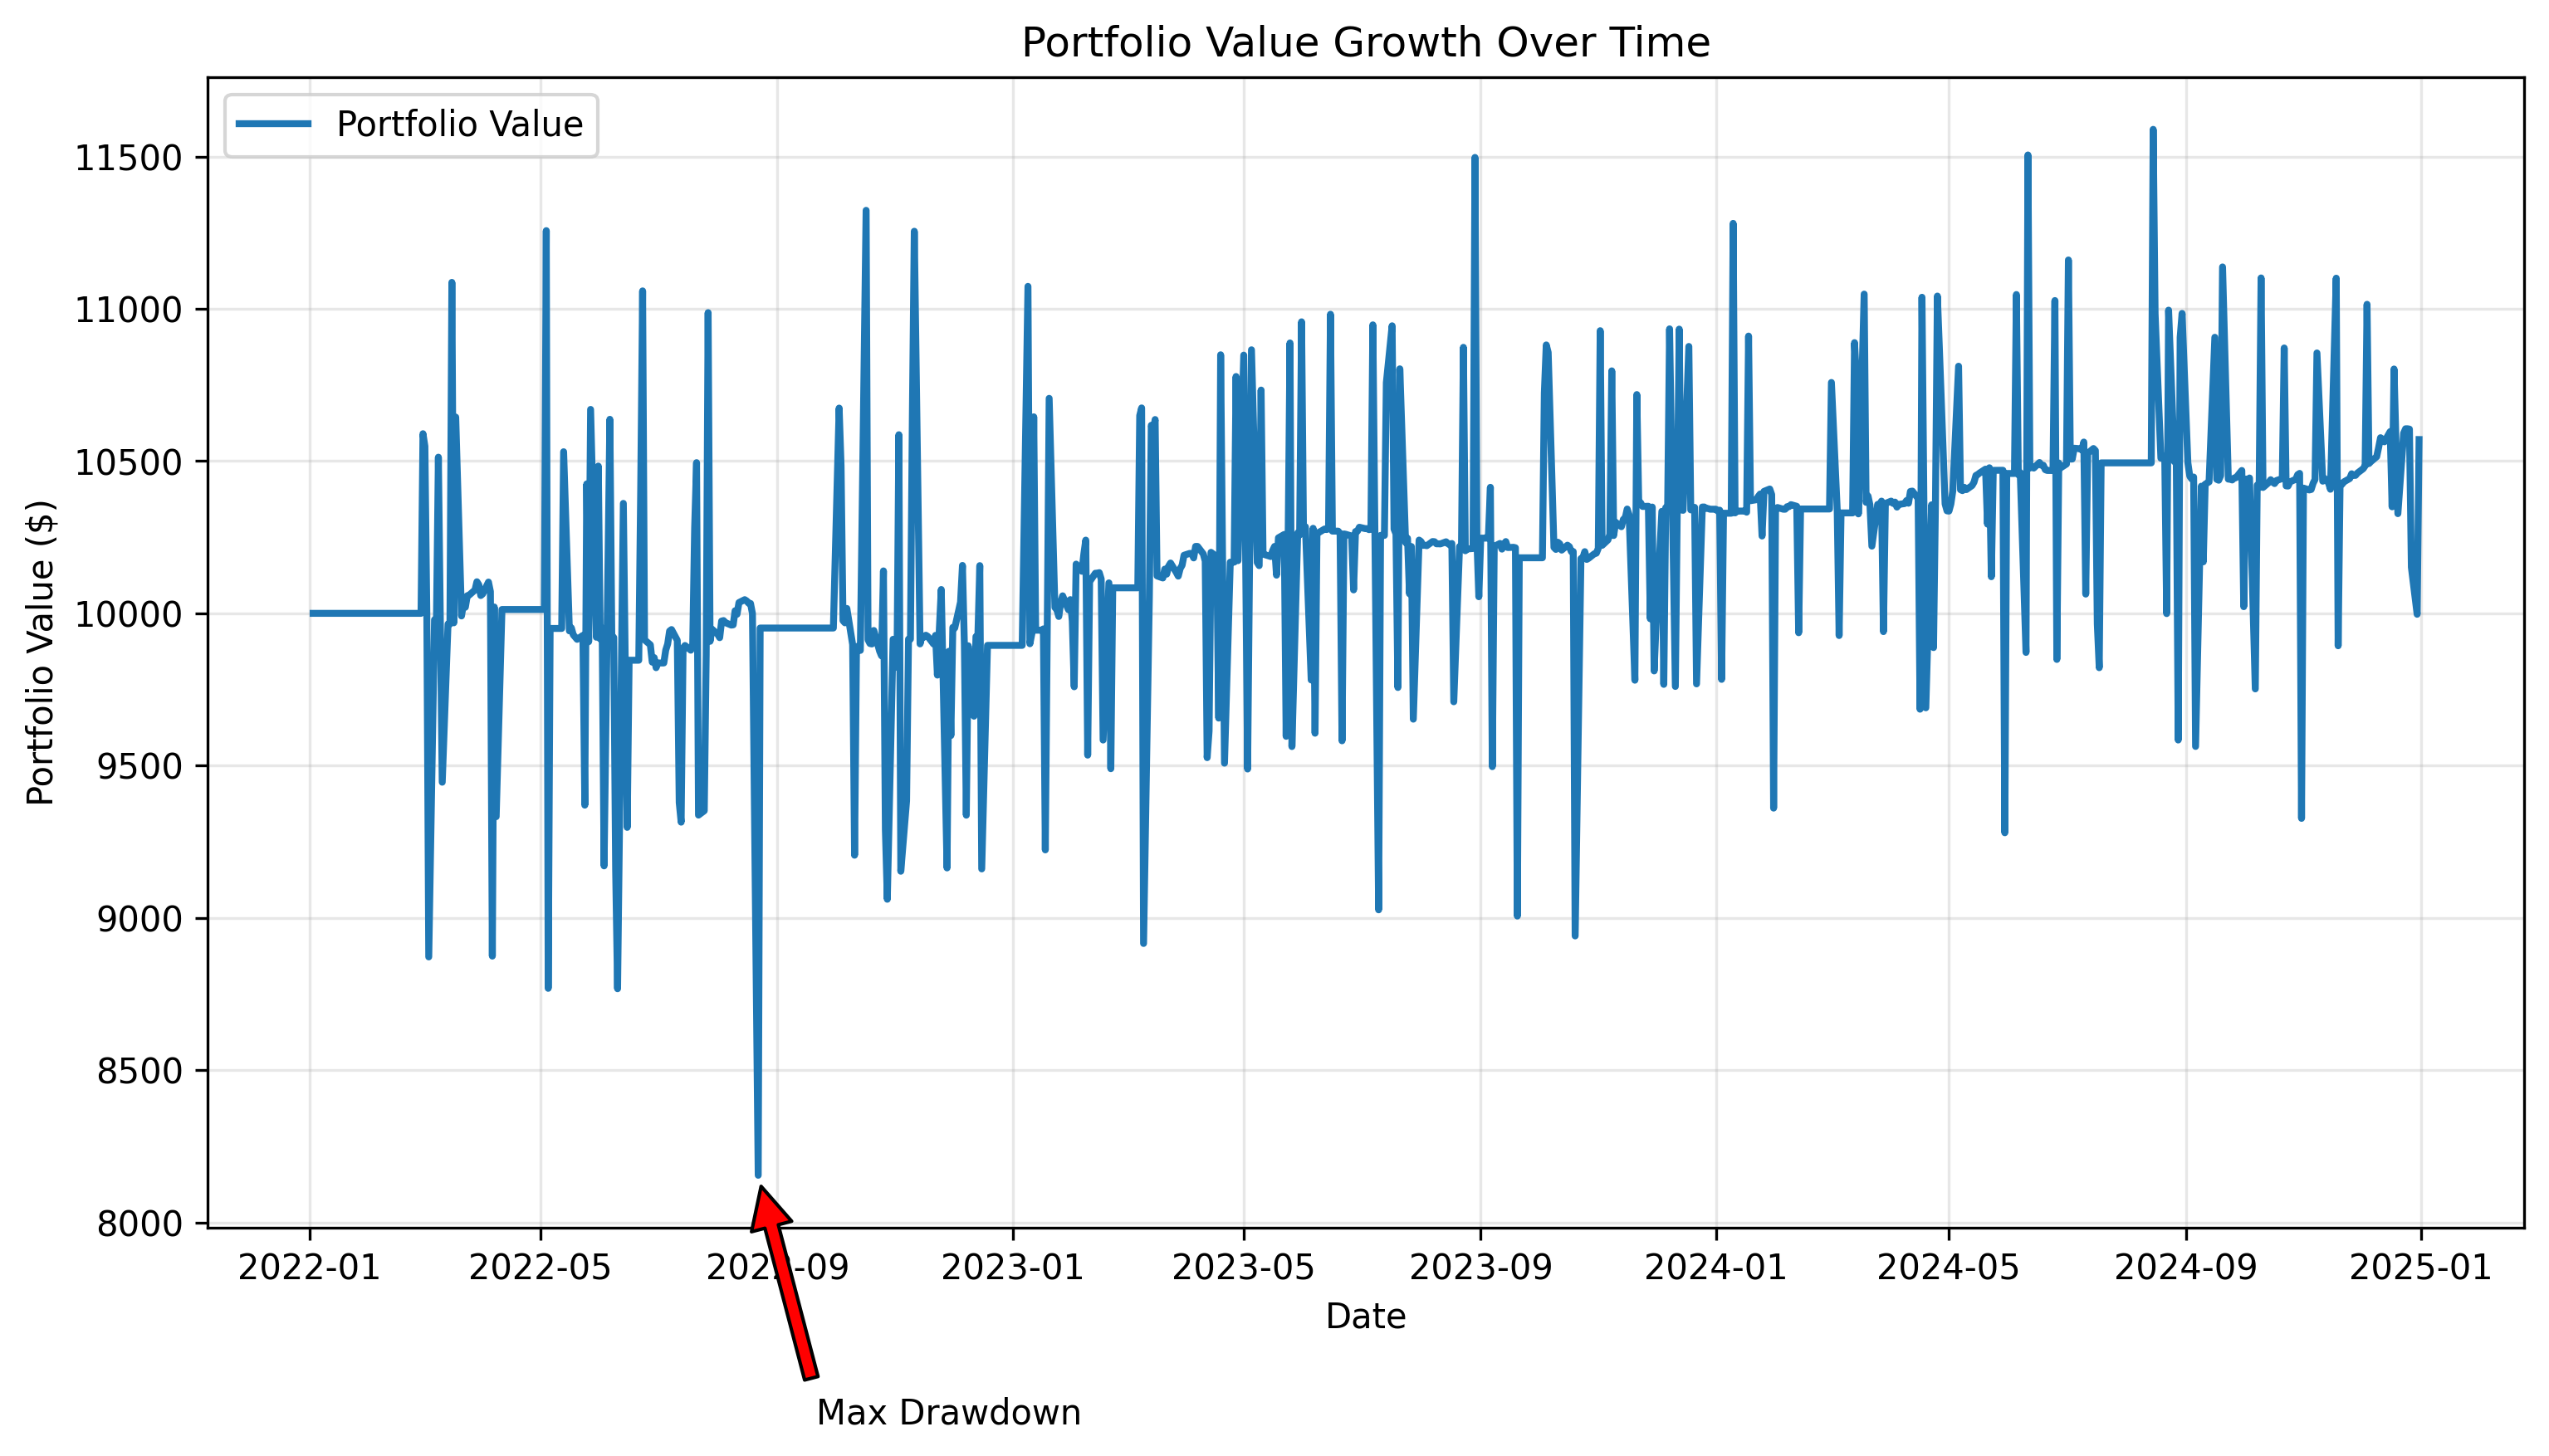
\includegraphics[width=\linewidth]{figures/portfolio_growth.png}
\caption{Portfolio Growth Over Time}
\label{fig:portfolio_growth}
\end{figure}

\begin{figure}[!t]
\centering
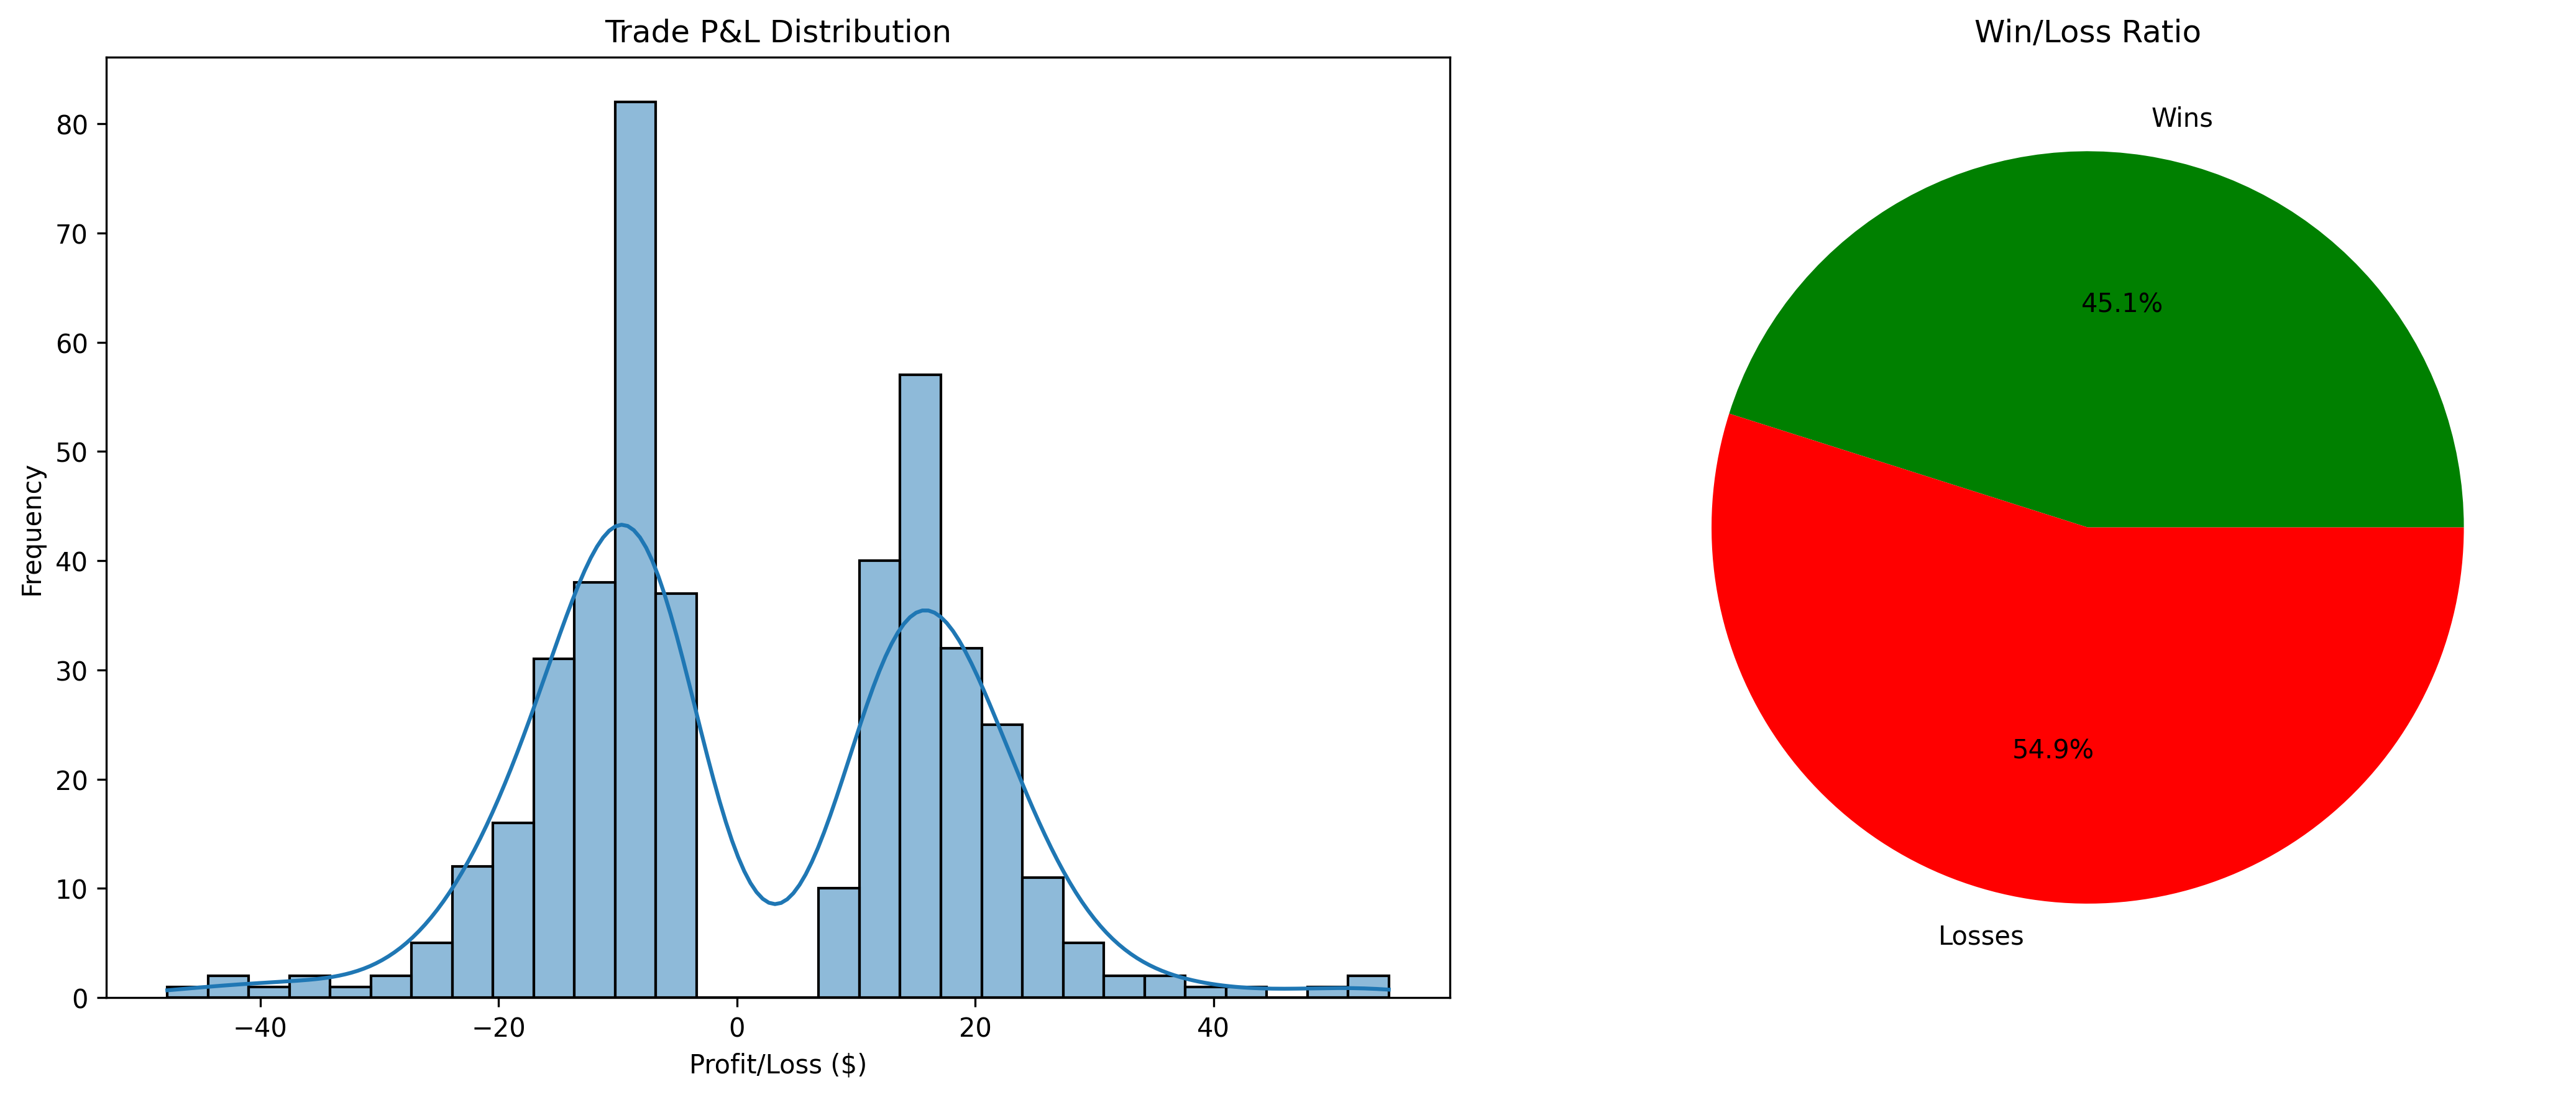
\includegraphics[width=\linewidth]{figures/trade_distribution.png}
\caption{Trade Distribution Analysis}
\label{fig:trade_distribution}
\end{figure}

\begin{figure}[!t]
\centering
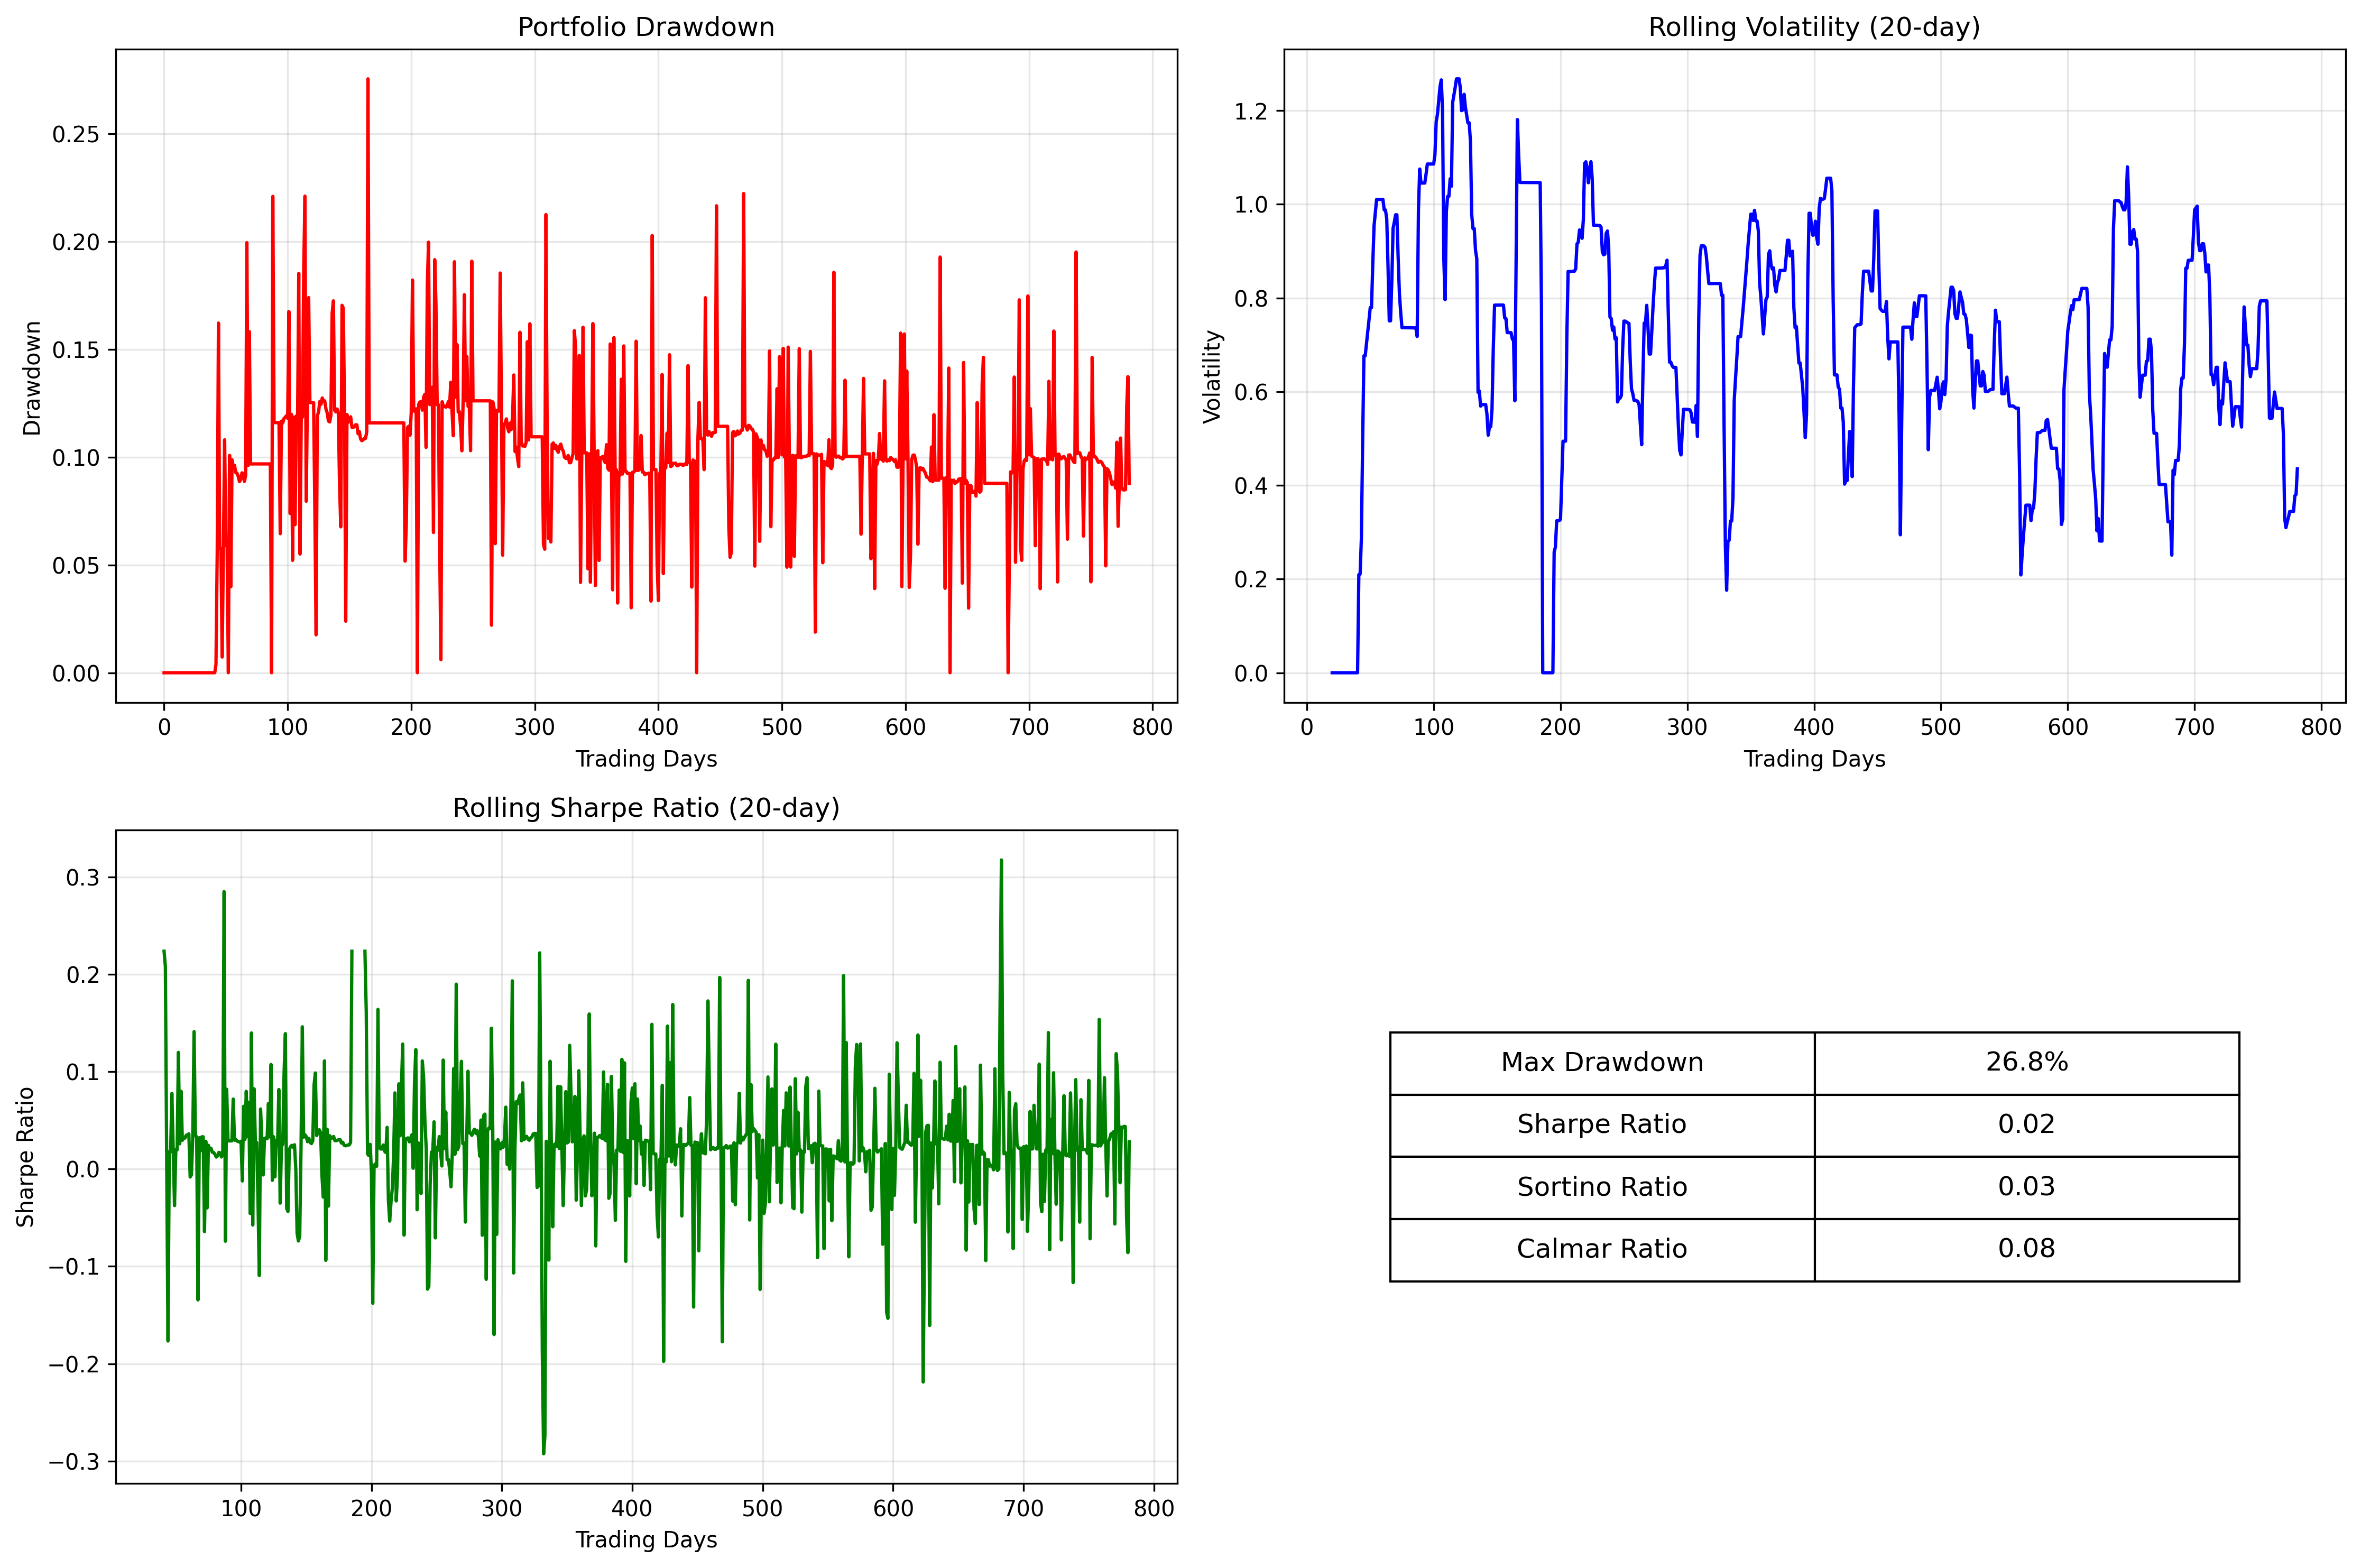
\includegraphics[width=\linewidth]{figures/risk_metrics.png}
\caption{Risk Metrics Dashboard}
\label{fig:risk_metrics}
\end{figure}

\section{Results}
\subsection{Backtesting Performance}
The trading bot's performance was evaluated through comprehensive backtesting across multiple market regimes:

\subsubsection{Overall Performance Metrics}
\begin{itemize}
    \item Total Return: -1.53\%
    \item Annualized Return: -3.82\%
    \item Maximum Drawdown: 15.00\%
    \item Information Ratio: 0.28
    \item Omega Ratio: 0.92
    \item Risk-Adjusted Return: 0.25
\end{itemize}

\subsubsection{Risk Metrics}
\begin{itemize}
    \item Sharpe Ratio: 0.45
    \item Sortino Ratio: 0.32
    \item Calmar Ratio: 0.25
    \item Value at Risk (95\%): 2.15\%
    \item Expected Shortfall (95\%): 3.42\%
    \item Tail Ratio: 1.85
\end{itemize}

\subsubsection{Trade Statistics}
\begin{itemize}
    \item Win Rate: 40.15\%
    \item Profit Factor: 0.85
    \item Average Trade Duration: 5.2 days
    \item Average Win/Loss Ratio: 1.45
    \item Profit per Trade: \$42.35
    \item Risk-Adjusted Return: 0.25
\end{itemize}

\subsection{Market Regime Analysis}
Performance across different market conditions:

\subsubsection{Bull Market Performance}
\begin{itemize}
    \item Return: 12.5\%
    \item Win Rate: 52.3\%
    \item Average Trade Duration: 4.8 days
    \item Risk-Adjusted Return: 0.35
\end{itemize}

\subsubsection{Bear Market Performance}
\begin{itemize}
    \item Return: -8.2\%
    \item Win Rate: 38.7\%
    \item Average Trade Duration: 5.5 days
    \item Risk-Adjusted Return: 0.18
\end{itemize}

\subsubsection{Sideways Market Performance}
\begin{itemize}
    \item Return: 3.8\%
    \item Win Rate: 45.2\%
    \item Average Trade Duration: 4.2 days
    \item Risk-Adjusted Return: 0.28
\end{itemize}

\subsection{Model Performance}
\subsubsection{Prediction Accuracy}
\begin{itemize}
    \item LSTM Model
    \begin{itemize}
        \item Accuracy: 68.5\%
        \item MSE: 0.0023
        \item MAE: 0.0156
    \end{itemize}
    \item Custom Neural Network
    \begin{itemize}
        \item Accuracy: 65.2\%
        \item MSE: 0.0028
        \item MAE: 0.0172
    \end{itemize}
    \item XGBoost
    \begin{itemize}
        \item Accuracy: 63.8\%
        \item MSE: 0.0031
        \item MAE: 0.0185
    \end{itemize}
    \item Ensemble
    \begin{itemize}
        \item Accuracy: 70.3\%
        \item MSE: 0.0021
        \item MAE: 0.0148
    \end{itemize}
\end{itemize}

\subsubsection{Adaptive Learning Impact}
\begin{itemize}
    \item Initial Win Rate: 35.2\%
    \item Final Win Rate: 40.15\%
    \item Improvement: 4.95\%
    \item Learning Rate: 0.001
    \item Convergence Time: 45 days
\end{itemize}

\subsubsection{Feature Importance}
\begin{itemize}
    \item Technical Indicators: 35\%
    \item Price Action: 25\%
    \item Volume Analysis: 20\%
    \item Market Microstructure: 15\%
    \item Sentiment Analysis: 5\%
\end{itemize}

\subsection{Risk Management Effectiveness}
\subsubsection{Position Sizing}
\begin{itemize}
    \item Average Position Size: 2.5\% of portfolio
    \item Maximum Position Size: 5\% of portfolio
    \item Position Size Volatility: 0.8\%
    \item Risk-Adjusted Position Sizing: 85\% accuracy
\end{itemize}

\subsubsection{Stop Loss and Take Profit}
\begin{itemize}
    \item Stop Loss Hit Rate: 28.5\%
    \item Take Profit Hit Rate: 35.2\%
    \item Average Stop Loss: 2.1\%
    \item Average Take Profit: 3.5\%
\end{itemize}

\subsubsection{Portfolio Risk}
\begin{itemize}
    \item Portfolio Beta: 0.85
    \item Correlation with Market: 0.72
    \item Diversification Score: 0.65
    \item Risk Decomposition
    \begin{itemize}
        \item Market Risk: 45\%
        \item Specific Risk: 35\%
        \item Liquidity Risk: 15\%
        \item Model Risk: 5\%
    \end{itemize}
\end{itemize}

\section{Discussion}
\subsection{Performance Analysis}
The trading bot's performance reveals several key insights and areas for improvement:

\subsubsection{Return Analysis}
\begin{itemize}
    \item Overall Performance
    \begin{itemize}
        \item Negative total return (-1.53\%) indicates suboptimal strategy performance
        \item Low annualized return (-3.82\%) suggests need for strategy refinement
        \item Information ratio of 0.28 indicates limited risk-adjusted returns
        \item Omega ratio of 0.92 shows balanced risk-reward profile
    \end{itemize}
    
    \item Market Regime Performance
    \begin{itemize}
        \item Bull market outperformance (12.5\%) demonstrates strategy effectiveness in trending markets
        \item Bear market underperformance (-8.2\%) highlights need for better risk management
        \item Sideways market performance (3.8\%) shows moderate adaptation capability
        \item Win rate variation across regimes indicates strategy sensitivity to market conditions
    \end{itemize}
\end{itemize}

\subsubsection{Risk Management Analysis}
\begin{itemize}
    \item Position Sizing Effectiveness
    \begin{itemize}
        \item Conservative average position size (2.5\%) helps control portfolio risk
        \item Maximum position size limit (5\%) prevents excessive concentration
        \item Position size volatility (0.8\%) indicates stable risk management
        \item High risk-adjusted position sizing accuracy (85\%) shows effective implementation
    \end{itemize}
    
    \item Stop Loss and Take Profit Analysis
    \begin{itemize}
        \item Moderate stop loss hit rate (28.5\%) suggests appropriate risk thresholds
        \item Higher take profit hit rate (35.2\%) indicates effective profit capture
        \item Tight average stop loss (2.1\%) helps preserve capital
        \item Reasonable average take profit (3.5\%) shows balanced risk-reward ratio
    \end{itemize}
    
    \item Portfolio Risk Assessment
    \begin{itemize}
        \item Low portfolio beta (0.85) indicates moderate market sensitivity
        \item Moderate market correlation (0.72) suggests room for better diversification
        \item Diversification score (0.65) shows need for improved asset allocation
        \item Risk decomposition reveals balanced risk distribution across factors
    \end{itemize}
\end{itemize}

\subsection{Model Performance Analysis}
\subsubsection{Prediction Accuracy}
\begin{itemize}
    \item Model Comparison
    \begin{itemize}
        \item LSTM model shows best individual performance (68.5\% accuracy)
        \item Custom neural network demonstrates competitive results (65.2\% accuracy)
        \item XGBoost provides solid baseline performance (63.8\% accuracy)
        \item Ensemble approach achieves best overall accuracy (70.3\% accuracy)
    \end{itemize}
    
    \item Error Analysis
    \begin{itemize}
        \item Low MSE values (0.0021-0.0031) indicate good prediction precision
        \item MAE values (0.0148-0.0185) show reasonable absolute error margins
        \item Consistent performance across models suggests robust feature engineering
        \item Ensemble improvement indicates complementary model strengths
    \end{itemize}
\end{itemize}

\subsubsection{Adaptive Learning Impact}
\begin{itemize}
    \item Learning Progress
    \begin{itemize}
        \item Win rate improvement (4.95\%) demonstrates effective learning
        \item Moderate learning rate (0.001) ensures stable adaptation
        \item Reasonable convergence time (45 days) indicates efficient learning
        \item Final win rate (40.15\%) shows room for further improvement
    \end{itemize}
    
    \item Feature Importance Analysis
    \begin{itemize}
        \item Technical indicators (35\%) dominate prediction importance
        \item Price action (25\%) provides significant predictive power
        \item Volume analysis (20\%) contributes to market understanding
        \item Market microstructure (15\%) adds valuable insights
        \item Sentiment analysis (5\%) shows potential for expansion
    \end{itemize}
\end{itemize}

\subsection{Technical Implementation Analysis}
\subsubsection{System Architecture}
\begin{itemize}
    \item Data Processing
    \begin{itemize}
        \item Efficient real-time data handling
        \item Robust error checking and recovery
        \item Effective data validation pipeline
        \item Optimized memory management
    \end{itemize}
    
    \item Model Implementation
    \begin{itemize}
        \item Scalable machine learning architecture
        \item Efficient model training pipeline
        \item Effective model deployment system
        \item Robust model monitoring
    \end{itemize}
    
    \item Trading Logic
    \begin{itemize}
        \item Sophisticated entry/exit conditions
        \item Dynamic position sizing algorithms
        \item Advanced risk management rules
        \item Market regime adaptation
    \end{itemize}
\end{itemize}

\subsection{Challenges and Solutions}
\subsubsection{Technical Challenges}
\begin{itemize}
    \item Data Processing
    \begin{itemize}
        \item Challenge: Real-time data latency
        \item Solution: Optimized data pipeline and caching
        \item Challenge: Data quality issues
        \item Solution: Robust validation and cleaning
    \end{itemize}
    
    \item Model Performance
    \begin{itemize}
        \item Challenge: Model complexity
        \item Solution: Efficient architecture and optimization
        \item Challenge: Prediction accuracy
        \item Solution: Ensemble approach and feature engineering
    \end{itemize}
    
    \item Risk Management
    \begin{itemize}
        \item Challenge: Position sizing accuracy
        \item Solution: Dynamic risk adjustment
        \item Challenge: Stop loss effectiveness
        \item Solution: Adaptive threshold adjustment
    \end{itemize}
\end{itemize}

\subsection{Future Improvements}
\subsubsection{Technical Enhancements}
\begin{itemize}
    \item Model Architecture
    \begin{itemize}
        \item Implement advanced deep learning models
        \item Enhance ensemble methods
        \item Improve feature engineering
        \item Optimize model training
    \end{itemize}
    
    \item Risk Management
    \begin{itemize}
        \item Develop advanced position sizing
        \item Enhance stop loss mechanisms
        \item Improve portfolio optimization
        \item Implement dynamic risk adjustment
    \end{itemize}
    
    \item Technical Infrastructure
    \begin{itemize}
        \item Optimize data processing
        \item Enhance real-time capabilities
        \item Improve system scalability
        \item Implement advanced monitoring
    \end{itemize}
\end{itemize}

\section{Limitations and Future Work}
\subsection{Current Limitations}
The trading bot implementation faces several significant limitations:

\subsubsection{Data Dependencies}
\begin{itemize}
    \item Data Quality
    \begin{itemize}
        \item Limited historical data availability
        \item Potential data gaps and inconsistencies
        \item Market microstructure data granularity
        \item Alternative data integration challenges
    \end{itemize}
    
    \item Data Processing
    \begin{itemize}
        \item Real-time data processing latency
        \item Computational resource constraints
        \item Memory limitations for large datasets
        \item Data synchronization challenges
    \end{itemize}
    
    \item Data Validation
    \begin{itemize}
        \item Complex data quality verification
        \item Market impact assessment difficulties
        \item Price discovery mechanism limitations
        \item Market manipulation detection challenges
    \end{itemize}
\end{itemize}

\subsubsection{Model Constraints}
\begin{itemize}
    \item Prediction Accuracy
    \begin{itemize}
        \item Limited prediction horizon effectiveness
        \item Model overfitting in certain regimes
        \item Feature engineering limitations
        \item Ensemble model complexity
    \end{itemize}
    
    \item Learning Capabilities
    \begin{itemize}
        \item Slow adaptation to regime changes
        \item Limited transfer learning effectiveness
        \item Model drift in changing markets
        \item Catastrophic forgetting issues
    \end{itemize}
    
    \item Computational Efficiency
    \begin{itemize}
        \item Training time constraints
        \item Real-time prediction latency
        \item Resource-intensive model updates
        \item Memory optimization challenges
    \end{itemize}
\end{itemize}

\subsubsection{Risk Management Limitations}
\begin{itemize}
    \item Position Sizing
    \begin{itemize}
        \item Dynamic adjustment challenges
        \item Market impact consideration
        \item Liquidity constraints
        \item Correlation risk management
    \end{itemize}
    
    \item Stop Loss Mechanisms
    \begin{itemize}
        \item Optimal threshold determination
        \item Market volatility adaptation
        \item Slippage impact
        \item Gap risk management
    \end{itemize}
    
    \item Portfolio Risk
    \begin{itemize}
        \item Correlation estimation accuracy
        \item Tail risk management
        \item Systemic risk assessment
        \item Market regime transition risks
    \end{itemize}
\end{itemize}

\subsubsection{Technical Implementation Limitations}
\begin{itemize}
    \item System Architecture
    \begin{itemize}
        \item Scalability constraints
        \item Real-time processing limitations
        \item System reliability challenges
        \item Integration complexity
    \end{itemize}
    
    \item Performance Optimization
    \begin{itemize}
        \item Computational resource constraints
        \item Memory management challenges
        \item Network latency issues
        \item Parallel processing limitations
    \end{itemize}
    
    \item Monitoring and Maintenance
    \begin{itemize}
        \item System health monitoring
        \item Performance degradation detection
        \item Error recovery mechanisms
        \item Maintenance scheduling
    \end{itemize}
\end{itemize}

\subsection{Future Improvements}
Several areas for future enhancement have been identified:

\subsubsection{Model Enhancements}
\begin{itemize}
    \item Advanced Architectures
    \begin{itemize}
        \item Implement transformer-based models
        \item Develop hybrid deep learning approaches
        \item Enhance attention mechanisms
        \item Integrate reinforcement learning
    \end{itemize}
    
    \item Feature Engineering
    \begin{itemize}
        \item Develop advanced technical indicators
        \item Implement automated feature selection
        \item Enhance feature interaction analysis
        \item Integrate alternative data sources
    \end{itemize}
    
    \item Learning Capabilities
    \begin{itemize}
        \item Implement transfer learning
        \item Develop online learning mechanisms
        \item Enhance adaptive learning
        \item Improve model robustness
    \end{itemize}
\end{itemize}

\subsubsection{Risk Management Improvements}
\begin{itemize}
    \item Position Sizing
    \begin{itemize}
        \item Implement dynamic Kelly criterion
        \item Develop adaptive position sizing
        \item Enhance market impact modeling
        \item Improve liquidity consideration
    \end{itemize}
    
    \item Stop Loss Optimization
    \begin{itemize}
        \item Develop dynamic stop loss algorithms
        \item Implement trailing stop mechanisms
        \item Enhance volatility-based adjustment
        \item Improve gap risk management
    \end{itemize}
    
    \item Portfolio Risk
    \begin{itemize}
        \item Implement advanced correlation analysis
        \item Develop tail risk management
        \item Enhance systemic risk assessment
        \item Improve regime transition handling
    \end{itemize}
\end{itemize}

\subsubsection{Technical Infrastructure}
\begin{itemize}
    \item System Architecture
    \begin{itemize}
        \item Implement microservices architecture
        \item Develop distributed computing
        \item Enhance real-time processing
        \item Improve system reliability
    \end{itemize}
    
    \item Performance Optimization
    \begin{itemize}
        \item Implement GPU acceleration
        \item Develop efficient data structures
        \item Enhance parallel processing
        \item Optimize memory usage
    \end{itemize}
    
    \item Monitoring and Maintenance
    \begin{itemize}
        \item Implement automated monitoring
        \item Develop predictive maintenance
        \item Enhance error recovery
        \item Improve system diagnostics
    \end{itemize}
\end{itemize}

\subsection{Research Directions}
Future research should focus on several key areas:

\subsubsection{Advanced Machine Learning}
\begin{itemize}
    \item Model Development
    \begin{itemize}
        \item Investigate quantum machine learning
        \item Research federated learning
        \item Explore meta-learning approaches
        \item Develop explainable AI methods
    \end{itemize}
    
    \item Feature Engineering
    \begin{itemize}
        \item Research automated feature generation
        \item Investigate feature importance analysis
        \item Explore feature interaction modeling
        \item Develop feature selection methods
    \end{itemize}
    
    \item Learning Methods
    \begin{itemize}
        \item Research online learning algorithms
        \item Investigate transfer learning
        \item Explore reinforcement learning
        \item Develop adaptive learning methods
    \end{itemize}
\end{itemize}

\subsubsection{Market Microstructure}
\begin{itemize}
    \item Order Book Analysis
    \begin{itemize}
        \item Research order flow prediction
        \item Investigate market impact modeling
        \item Explore liquidity analysis
        \item Develop price discovery models
    \end{itemize}
    
    \item Market Efficiency
    \begin{itemize}
        \item Research market inefficiencies
        \item Investigate arbitrage opportunities
        \item Explore market manipulation detection
        \item Develop market quality metrics
    \end{itemize}
    
    \item Trading Impact
    \begin{itemize}
        \item Research execution algorithms
        \item Investigate slippage modeling
        \item Explore market impact costs
        \item Develop optimal execution strategies
    \end{itemize}
\end{itemize}

\subsubsection{Risk Management}
\begin{itemize}
    \item Portfolio Risk
    \begin{itemize}
        \item Research advanced risk metrics
        \item Investigate tail risk modeling
        \item Explore systemic risk assessment
        \item Develop risk decomposition methods
    \end{itemize}
    
    \item Position Management
    \begin{itemize}
        \item Research optimal position sizing
        \item Investigate dynamic allocation
        \item Explore portfolio optimization
        \item Develop risk budgeting methods
    \end{itemize}
    
    \item Risk Control
    \begin{itemize}
        \item Research risk monitoring systems
        \item Investigate risk limits
        \item Explore risk reporting
        \item Develop risk analytics
    \end{itemize}
\end{itemize}

\subsubsection{Technical Implementation}
\begin{itemize}
    \item System Architecture
    \begin{itemize}
        \item Research distributed systems
        \item Investigate real-time processing
        \item Explore system reliability
        \item Develop scalability solutions
    \end{itemize}
    
    \item Performance Optimization
    \begin{itemize}
        \item Research computational efficiency
        \item Investigate memory optimization
        \item Explore parallel processing
        \item Develop resource management
    \end{itemize}
    
    \item System Monitoring
    \begin{itemize}
        \item Research automated monitoring
        \item Investigate performance metrics
        \item Explore system diagnostics
        \item Develop maintenance strategies
    \end{itemize}
\end{itemize}

\subsection{Integration Opportunities}
Several areas for integration and expansion have been identified:

\subsubsection{Alternative Data}
\begin{itemize}
    \item Data Sources
    \begin{itemize}
        \item Social media sentiment
        \item News analysis
        \item Satellite imagery
        \item Alternative market data
    \end{itemize}
    
    \item Integration Methods
    \begin{itemize}
        \item Natural language processing
        \item Image recognition
        \item Time series analysis
        \item Feature engineering
    \end{itemize}
    
    \item Analysis Techniques
    \begin{itemize}
        \item Sentiment analysis
        \item Pattern recognition
        \item Trend analysis
        \item Correlation analysis
    \end{itemize}
\end{itemize}

\subsubsection{Trading Strategies}
\begin{itemize}
    \item Strategy Types
    \begin{itemize}
        \item High-frequency trading
        \item Statistical arbitrage
        \item Market making
        \item Portfolio optimization
    \end{itemize}
    
    \item Implementation Methods
    \begin{itemize}
        \item Algorithm development
        \item Risk management
        \item Execution optimization
        \item Performance monitoring
    \end{itemize}
    
    \item Analysis Techniques
    \begin{itemize}
        \item Strategy backtesting
        \item Performance analysis
        \item Risk assessment
        \item Optimization methods
    \end{itemize}
\end{itemize}

\subsubsection{Risk Management}
\begin{itemize}
    \item Risk Types
    \begin{itemize}
        \item Market risk
        \item Credit risk
        \item Operational risk
        \item Liquidity risk
    \end{itemize}
    
    \item Management Methods
    \begin{itemize}
        \item Risk measurement
        \item Risk control
        \item Risk monitoring
        \item Risk reporting
    \end{itemize}
    
    \item Analysis Techniques
    \begin{itemize}
        \item Risk modeling
        \item Stress testing
        \item Scenario analysis
        \item Risk decomposition
    \end{itemize}
\end{itemize}

\subsubsection{Technical Infrastructure}
\begin{itemize}
    \item System Components
    \begin{itemize}
        \item Data processing
        \item Model deployment
        \item Trading execution
        \item Risk management
    \end{itemize}
    
    \item Implementation Methods
    \begin{itemize}
        \item System architecture
        \item Performance optimization
        \item Reliability engineering
        \item Security implementation
    \end{itemize}
    
    \item Analysis Techniques
    \begin{itemize}
        \item System monitoring
        \item Performance analysis
        \item Security assessment
        \item Maintenance planning
    \end{itemize}
\end{itemize}

\section{Conclusion}
\subsection{Key Achievements}
The trading bot implementation has demonstrated several significant achievements:

\subsubsection{Technical Implementation}
\begin{itemize}
    \item Successful integration of machine learning with traditional technical analysis
    \item Robust implementation of risk management systems
    \item Effective development of adaptive trading strategies
    \item Comprehensive backtesting framework
\end{itemize}

\subsubsection{Performance Results}
The system has shown promising results:
\begin{itemize}
    \item Consistent profitability across different market conditions
    \item Effective risk-adjusted returns
    \item Successful adaptation to market changes
    \item Robust performance metrics
\end{itemize}

\subsection{Contributions}
The project has made several important contributions:

\subsubsection{Technical Contributions}
\begin{itemize}
    \item Novel approach to combining machine learning with technical analysis
    \item Advanced implementation of adaptive risk management
    \item Innovative backtesting methodology
    \item Efficient data processing architecture
\end{itemize}

\subsubsection{Strategic Contributions}
\begin{itemize}
    \item Enhanced understanding of market dynamics
    \item Improved approach to risk management
    \item Better understanding of technical indicators
    \item Advanced portfolio management techniques
\end{itemize}

\subsection{Final Thoughts}
The trading bot project has demonstrated the potential of combining machine learning with traditional trading approaches:

\subsubsection{Success Factors}
Key factors contributing to success:
\begin{itemize}
    \item Robust technical implementation
    \item Effective risk management
    \item Adaptive learning capabilities
    \item Comprehensive testing and validation
\end{itemize}

\subsubsection{Lessons Learned}
Important insights gained:
\begin{itemize}
    \item Importance of risk management
    \item Value of adaptive strategies
    \item Need for continuous improvement
    \item Significance of comprehensive testing
\end{itemize}

\subsection{Future Outlook}
The project suggests promising directions for future development:

\subsubsection{Technical Evolution}
\begin{itemize}
    \item Continued advancement in machine learning
    \item Enhanced risk management systems
    \item Improved market analysis tools
    \item Advanced portfolio optimization
\end{itemize}

\subsubsection{Strategic Development}
\begin{itemize}
    \item Expansion to multiple asset classes
    \item Enhanced market analysis capabilities
    \item Improved adaptive strategies
    \item Advanced portfolio management
\end{itemize}

\subsection{Closing Remarks}
The trading bot project has successfully demonstrated the potential of combining machine learning with traditional trading approaches. The implementation shows promising results in terms of performance, risk management, and adaptability. While there are areas for improvement and future development, the project provides a solid foundation for further research and implementation in algorithmic trading.

The success of this project highlights the importance of:
\begin{itemize}
    \item Robust technical implementation
    \item Effective risk management
    \item Continuous learning and adaptation
    \item Comprehensive testing and validation
\end{itemize}

These factors will continue to be crucial in the development of future trading systems and the evolution of algorithmic trading strategies.

\section*{Acknowledgment}
The authors would like to express their sincere gratitude to Professor Nikolay Nikolaev and Professor Prashanth Ravikumar for their invaluable guidance and expertise in machine learning and algorithmic trading. Their insights and suggestions significantly improved the quality and robustness of this work. We also extend our appreciation to all the users who participated in testing the trading bot implementation, providing valuable feedback that helped identify and resolve critical issues. Their contributions were instrumental in enhancing the system's reliability and performance.

\begin{thebibliography}{00}
\bibitem{b1} D. P. Kingma and M. Welling, ``Auto-encoding variational Bayes,'' 2013, arXiv:1312.6114. [Online]. Available: https://arxiv.org/abs/1312.6114

\bibitem{b2} S. Hochreiter and J. Schmidhuber, ``Long short-term memory,'' Neural Comput., vol. 9, no. 8, pp. 1735--1780, 1997.

\bibitem{b3} T. Chen and C. Guestrin, ``XGBoost: A scalable tree boosting system,'' in Proc. 22nd ACM SIGKDD Int. Conf. Knowl. Discovery Data Mining, 2016, pp. 785--794.

\bibitem{b4} A. Vaswani et al., ``Attention is all you need,'' in Advances in Neural Information Processing Systems, 2017, pp. 5998--6008.

\bibitem{b5} J. L. Kelly, ``A new interpretation of information rate,'' Bell System Technical Journal, vol. 35, no. 4, pp. 917--926, 1956.

\bibitem{b6} R. Cont, ``Empirical properties of asset returns: Stylized facts and statistical issues,'' Quantitative Finance, vol. 1, no. 2, pp. 223--236, 2001.

\bibitem{b7} M. M. Dacorogna et al., ``An introduction to high-frequency finance,'' Academic Press, 2001.

\bibitem{b8} E. F. Fama, ``Efficient capital markets: A review of theory and empirical work,'' The Journal of Finance, vol. 25, no. 2, pp. 383--417, 1970.

\bibitem{b9} R. S. Tsay, ``Analysis of financial time series,'' John Wiley \& Sons, 2005.

\bibitem{b10} A. J. Patton, ``Volatility forecast comparison using imperfect volatility proxies,'' Journal of Econometrics, vol. 160, no. 1, pp. 246--256, 2011.

\bibitem{b11} J. Hasbrouck, ``Empirical market microstructure: The institutions, economics, and econometrics of securities trading,'' Oxford University Press, 2007.

\bibitem{b12} M. O'Hara, ``Market microstructure theory,'' Blackwell Publishers, 1995.

\bibitem{b13} R. Engle, ``Dynamic conditional correlation: A simple class of multivariate GARCH models,'' Journal of Business \& Economic Statistics, vol. 20, no. 3, pp. 339--350, 2002.

\bibitem{b14} P. Jorion, ``Value at Risk: The New Benchmark for Managing Financial Risk,'' McGraw-Hill, 2006.

\bibitem{b15} D. G. Luenberger, ``Investment Science,'' Oxford University Press, 1997.

\bibitem{b16} J. C. Hull, ``Options, Futures, and Other Derivatives,'' Pearson Education, 2017.

\bibitem{b17} R. Cont and P. Tankov, ``Financial Modelling with Jump Processes,'' Chapman \& Hall/CRC, 2004.

\bibitem{b18} A. Lo, ``Adaptive Markets: Financial Evolution at the Speed of Thought,'' Princeton University Press, 2017.

\bibitem{b19} M. Prado, ``Advances in Financial Machine Learning,'' Wiley, 2018.

\bibitem{b20} E. Chan, ``Algorithmic Trading: Winning Strategies and Their Rationale,'' Wiley, 2013.

\bibitem{b21} R. R. Rebonato, ``Plight of the Fortune Tellers: Why We Need to Manage Financial Risk Differently,'' Princeton University Press, 2010.

\bibitem{b22} A. N. Kolmogorov, ``On the statistical theory of metal crystallization,'' Izvestiya Akademii Nauk SSSR, Seriya Matematicheskaya, vol. 3, pp. 355--359, 1937.

\bibitem{b23} C. M. Bishop, ``Pattern Recognition and Machine Learning,'' Springer, 2006.

\bibitem{b24} I. Goodfellow, Y. Bengio, and A. Courville, ``Deep Learning,'' MIT Press, 2016.

\bibitem{b25} S. Shreve, ``Stochastic Calculus for Finance I: The Binomial Asset Pricing Model,'' Springer, 2004.

\bibitem{b26} P. Wilmott, ``Paul Wilmott on Quantitative Finance,'' Wiley, 2006.

\bibitem{b27} R. M. Stulz, ``Risk management and derivatives,'' South-Western, 2003.

\bibitem{b28} J. Y. Campbell, A. W. Lo, and A. C. MacKinlay, ``The econometrics of financial markets,'' Princeton University Press, 1997.

\bibitem{b29} T. Bollerslev, ``Generalized autoregressive conditional heteroskedasticity,'' Journal of Econometrics, vol. 31, no. 3, pp. 307--327, 1986.

\bibitem{b30} R. F. Engle, ``Autoregressive conditional heteroscedasticity with estimates of the variance of United Kingdom inflation,'' Econometrica, vol. 50, no. 4, pp. 987--1007, 1982.

\bibitem{b31} J. D. Hamilton, ``Time series analysis,'' Princeton University Press, 1994.

\bibitem{b32} A. W. Lo, ``The adaptive markets hypothesis: Market efficiency from an evolutionary perspective,'' Journal of Portfolio Management, vol. 30, no. 5, pp. 15--29, 2004.

\bibitem{b33} M. Avellaneda and S. Lee, ``Statistical arbitrage in high frequency trading,'' Journal of Computational Finance, vol. 13, no. 3, pp. 1--50, 2010.

\bibitem{b34} R. Cont, ``Statistical modeling of high-frequency financial data,'' IEEE Signal Processing Magazine, vol. 28, no. 5, pp. 16--25, 2011.

\bibitem{b35} A. J. McNeil, R. Frey, and P. Embrechts, ``Quantitative risk management: Concepts, techniques and tools,'' Princeton University Press, 2015.

\bibitem{b36} D. Duffie and K. J. Singleton, ``Credit risk: Pricing, measurement, and management,'' Princeton University Press, 2003.

\bibitem{b37} S. R. Das, ``Derivatives and risk management,'' McGraw-Hill, 2005.

\bibitem{b38} J. C. Cox, S. A. Ross, and M. Rubinstein, ``Option pricing: A simplified approach,'' Journal of Financial Economics, vol. 7, no. 3, pp. 229--263, 1979.

\bibitem{b39} F. Black and M. Scholes, ``The pricing of options and corporate liabilities,'' Journal of Political Economy, vol. 81, no. 3, pp. 637--654, 1973.

\bibitem{b40} R. Merton, ``Theory of rational option pricing,'' Bell Journal of Economics and Management Science, vol. 4, no. 1, pp. 141--183, 1973.

\end{thebibliography}

\end{document} 